%%%%%%%%%%%%%%%%%%%%%%%%%%%%%%%%%%%%%%%%%%%%%%%%%%%%%%%%%%%%%%%%%%%%%%%%%%%%%%%%%%
\begin{frame}[fragile]\frametitle{}
\begin{center}
{\Large Background}
\end{center}
\end{frame}

%%%%%%%%%%%%%%%%%%%%%%%%%%%%%%%%%%%%%%%%%%%%%%%%%%%%%%%%%%%
\begin{frame}[fragile]\frametitle{Progression}

Models for prediction:

\begin{itemize}
\item On data, derive features, put statistical techniques like regression. One model per task. That's Machine Learning.
\item Feed raw data, employ neural networks. One model per task. That's Deep Learning.
\item Use Text data, get embeddings, use ML/DL, say for classification. One model per task. That's Natural Language Processing.
\item Train neural network on large corpus, store weights and architecture, then add final layers for say classification on custom data+labels. That's Pretrained model. One model, many tasks.
\item Train Large Language Model, just supply instructions on what to do, works. One model many tasks. Zero-shot, few-shots.
\end{itemize}

{\tiny (More info at SaaS LLM https://medium.com/google-developer-experts/saasgpt-84ba80265d0f)}

\end{frame}


%%%%%%%%%%%%%%%%%%%%%%%%%%%%%%%%%%%%%%%%%%%%%%%%%%%%%%%%%%%
\begin{frame}[fragile]\frametitle{New Programming Language?}

\begin{center}

\includegraphics[width=0.8\linewidth,keepaspectratio]{promptengg1}

{\tiny (Ref: Prompt Engineering Sudalai Rajkumar)}

\end{center}				

\end{frame}



%%%%%%%%%%%%%%%%%%%%%%%%%%%%%%%%%%%%%%%%%%%%%%%%%%%%%%%%%%%
\begin{frame}[fragile]\frametitle{What is Prompt Engineering?}

Prompt engineering is a NLP concept that involves discovering inputs that yield desirable or useful results


\begin{center}
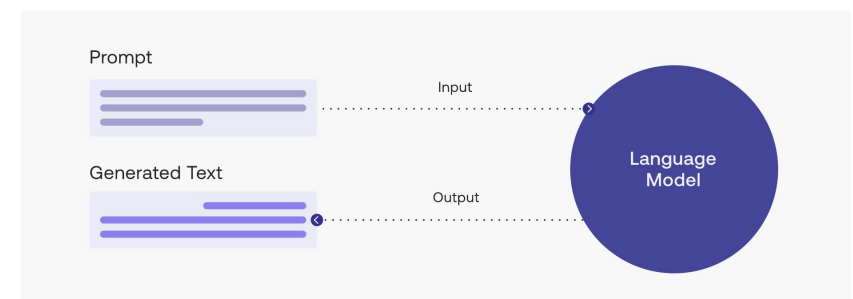
\includegraphics[width=\linewidth,keepaspectratio]{promptengg2}

{\tiny (Ref: Cohere https://docs.cohere.ai/docs/prompt-engineering)}

\end{center}				
			
			

\end{frame}



%%%%%%%%%%%%%%%%%%%%%%%%%%%%%%%%%%%%%%%%%%%%%%%%%%%%%%%%%%%
\begin{frame}[fragile]\frametitle{What is a Language Models?}

\begin{itemize}
\item While typing SMS, have you seen it suggests next word?
\item While typing email, have you seen next few words are suggested?
\item How does it suggest? (suggestions are not random, right?)
\item In the past, for ``Lets go for a \ldots', if you have typed 'coffee' 15 times, 'movie' say 4 times, then it learns that. Machine/Statistical Learning.
\item Next time, when you type ``Lets go for a '', what will be suggested? why?
\item This is called Language Model. Predicting the next word. When done continuously, one after other, it spits sentence, called Generative Model.
\end{itemize}	

\begin{center}
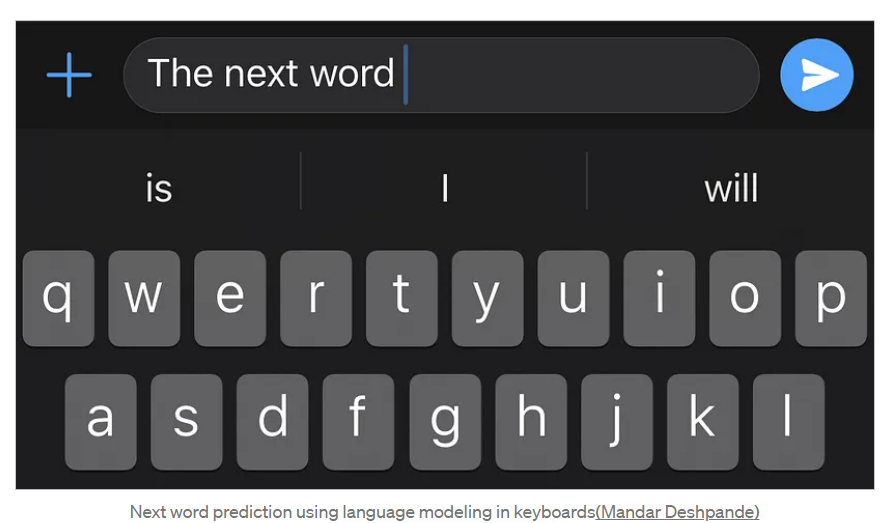
\includegraphics[width=0.6\linewidth,keepaspectratio]{chatgpt34}
\end{center}		

\end{frame}

%%%%%%%%%%%%%%%%%%%%%%%%%%%%%%%%%%%%%%%%%%%%%%%%%%%%%%%%%%%
\begin{frame}[fragile]\frametitle{Evolution of Language Models}

Language Models can be statistical (frequency based) or Machine/Deep Learning (supervised) based. Simple to complex.

\begin{center}
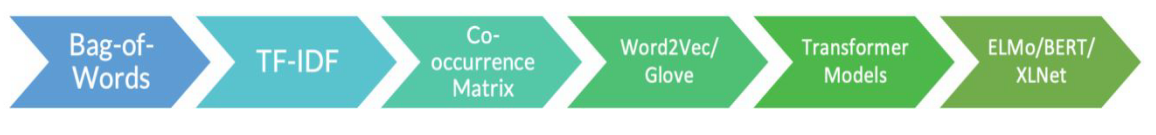
\includegraphics[width=\linewidth,keepaspectratio]{chatgpt30}
\end{center}				
{\tiny (Ref: Analytics Vidhya https://editor.analyticsvidhya.com/uploads/59483evolution\_of\_NLP.png)}

\end{frame}

%%%%%%%%%%%%%%%%%%%%%%%%%%%%%%%%%%%%%%%%%%%%%%%%%%%%%%%%%%%
\begin{frame}[fragile]\frametitle{Large Language Models - Comparison}

\begin{center}
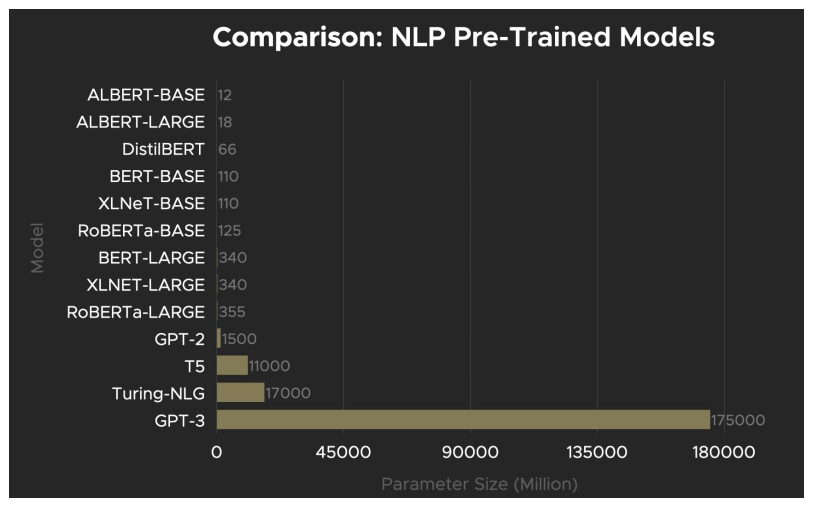
\includegraphics[width=\linewidth,keepaspectratio]{chatgpt31}
\end{center}				
{\tiny (Ref: Deus.ai https://www.deus.ai/post/gpt-3-what-is-all-the-excitement-about)}

\end{frame}

%%%%%%%%%%%%%%%%%%%%%%%%%%%%%%%%%%%%%%%%%%%%%%%%%%%%%%%%%%%
\begin{frame}[fragile]\frametitle{What is Prompt Engineering?}

How to talk to AI to get it to do what you want


\begin{center}
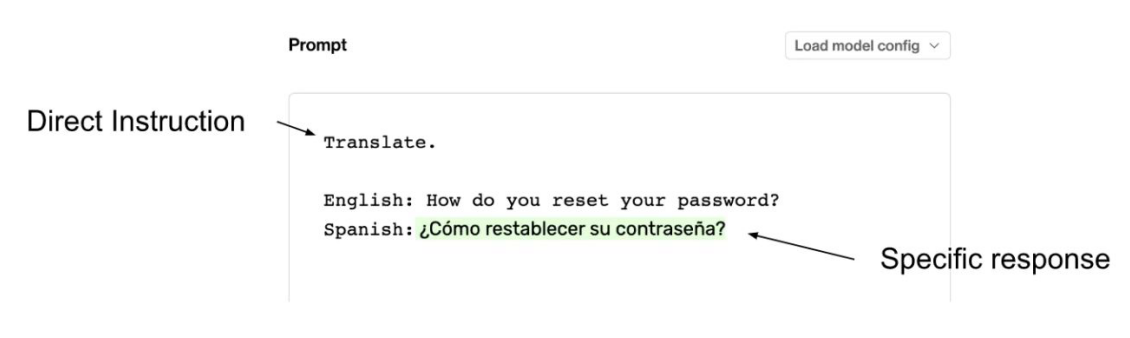
\includegraphics[width=\linewidth,keepaspectratio]{promptengg3}

{\tiny (Ref: Human Loop https://humanloop.com/blog/prompt-engineering-101)}

\end{center}				
			
			

\end{frame}

%%%%%%%%%%%%%%%%%%%%%%%%%%%%%%%%%%%%%%%%%%%%%%%%%%%%%%%%%%%
\begin{frame}[fragile]\frametitle{What is Prompt Engineering?}

But need to tell, for sure, else, nothing


\begin{center}
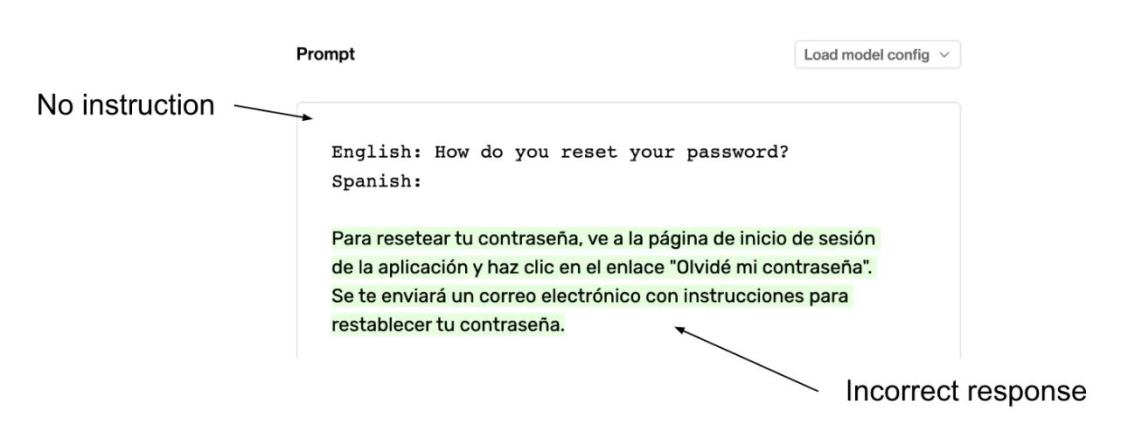
\includegraphics[width=\linewidth,keepaspectratio]{promptengg4}

{\tiny (Ref: Human Loop https://humanloop.com/blog/prompt-engineering-101)}

\end{center}				

\end{frame}


%%%%%%%%%%%%%%%%%%%%%%%%%%%%%%%%%%%%%%%%%%%%%%%%%%%%%%%%%%%
\begin{frame}[fragile]\frametitle{What is Prompt Engineering?}

\begin{itemize}
\item For prompt \lstinline|What is 1,000,000 * 9,000?| GPT-3 (text-davinci-002) (an AI) sometimes answers 9,000,000 (incorrect). This is where prompt engineering comes in.
\item If, instead of asking What is \lstinline|1,000,000 * 9,000?|, we ask \lstinline|What is 1,000,000 * 9,000? Make sure to put the right amount of zeros, even if there are many:|, GPT-3 will answer 9,000,000,000 (correct). 
\item Why is this the case? Why is the additional specification of the number of zeros necessary for the AI to get the right answer? How can we create prompts that yield optimal results on our task? 			
\item That's Prompt Engineering.
\end{itemize}

{\tiny (Ref: https://learnprompting.org/docs/basics/prompting)}
\end{frame}

%%%%%%%%%%%%%%%%%%%%%%%%%%%%%%%%%%%%%%%%%%%%%%%%%%%%%%%%%%%%%%%%%%%%%%%%%%%%%%%%%%
\begin{frame}[fragile]\frametitle{}
\begin{center}
{\Large Concepts}
\end{center}
\end{frame}



%%%%%%%%%%%%%%%%%%%%%%%%%%%%%%%%%%%%%%%%%%%%%%%%%%%%%%%%%%%
\begin{frame}[fragile]\frametitle{Elements of Prompt}

A prompt is composed of:

\begin{center}
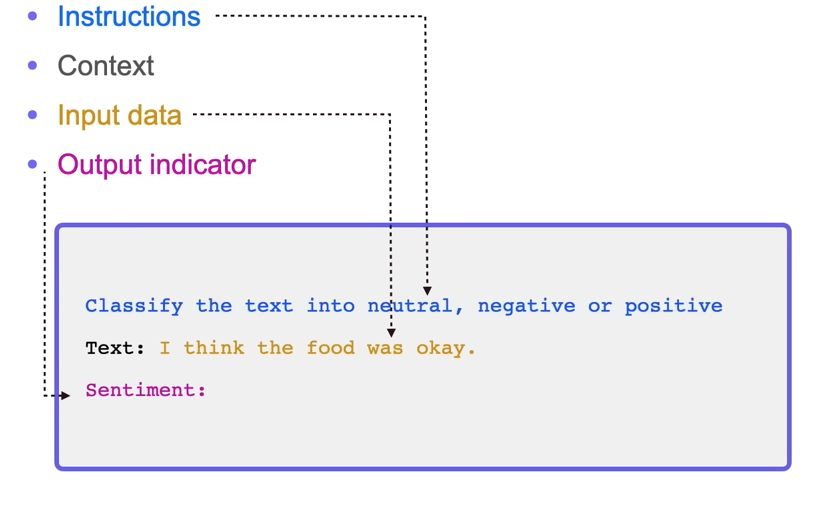
\includegraphics[width=0.8\linewidth,keepaspectratio]{promptengg28}

{\tiny (Ref: Prompt Engineering Overview - Elvis Saravia)}

\end{center}		
		
\end{frame}


%%%%%%%%%%%%%%%%%%%%%%%%%%%%%%%%%%%%%%%%%%%%%%%%%%%%%%%%%%%
\begin{frame}[fragile]\frametitle{Settings of Prompt}

\begin{itemize}
\item 'temperature':  before applying the softmax function, temperature is used scale the logits. With it, creativity or variability is allowed. If you re-run the prompt, with 0, no change, but with 1, lots of variation. Default is 0.7. With a temperature between 0 and 1, we can control the randomness and creativity of the model's predictions. Temperature defines how likely it is to choose less probable words. T=0 gives the same response every time because there's a 0% chance to choose any word but the most likely. T=1 just picks based on the model's base confidence.
\item 'top\_p' or 'nucleus sampling': specifies a sampling threshold during inference time, words passing the threshold are sampled for the output. Top-p goes for a minimal set of words, the probability of which does not exceed exceeds p. In practice, this means the following: if you choose reasonably high p, like 0.9, you would likely get a set of the most likely words for the model to choose from
\item Like the temperature, the top p parameter controls the randomness and originality of the model.
\item OpenAI documentation recommends using either one parameter or the other and setting the unused parameter to the neutral case, i.e. 1.0.
\end{itemize}
		
\end{frame}




%%%%%%%%%%%%%%%%%%%%%%%%%%%%%%%%%%%%%%%%%%%%%%%%%%%%%%%%%%%
\begin{frame}[fragile]\frametitle{Example: Prompting by Instruction}

\begin{center}
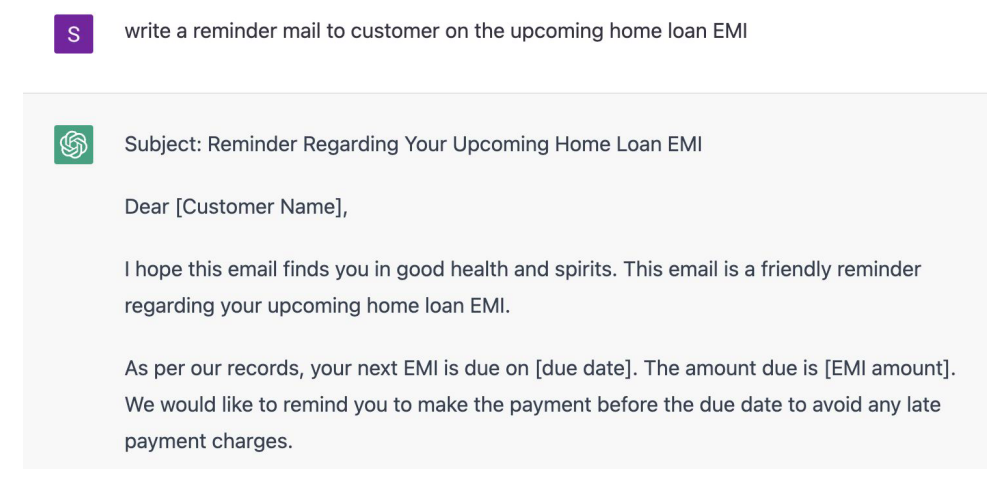
\includegraphics[width=\linewidth,keepaspectratio]{promptengg7}

{\tiny (Ref: Cohere https://txt.cohere.ai/generative-ai-part-1/)}

\end{center}		

\end{frame}

%%%%%%%%%%%%%%%%%%%%%%%%%%%%%%%%%%%%%%%%%%%%%%%%%%%%%%%%%%%
\begin{frame}[fragile]\frametitle{Prompting by Examples}

\begin{center}
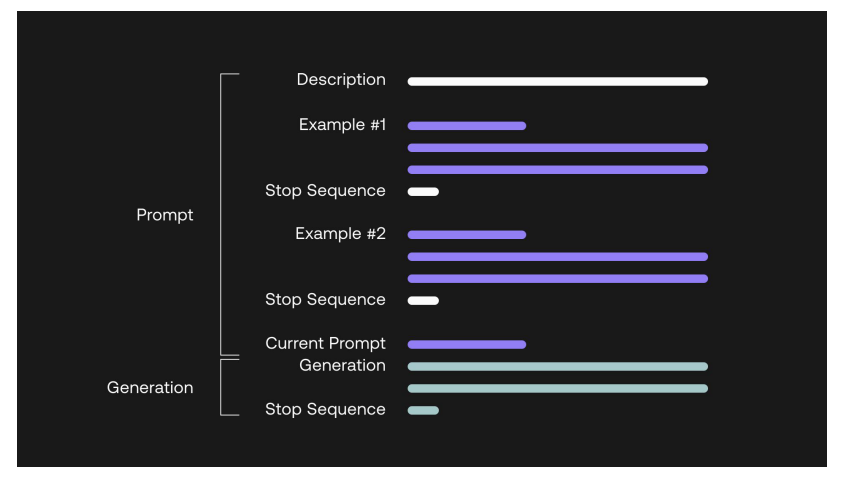
\includegraphics[width=\linewidth,keepaspectratio]{promptengg8}

{\tiny (Ref: Cohere https://txt.cohere.ai/generative-ai-part-1/)}

\end{center}		
		


\end{frame}

%%%%%%%%%%%%%%%%%%%%%%%%%%%%%%%%%%%%%%%%%%%%%%%%%%%%%%%%%%%
\begin{frame}[fragile]\frametitle{Example: Prompting by Examples}

\begin{center}
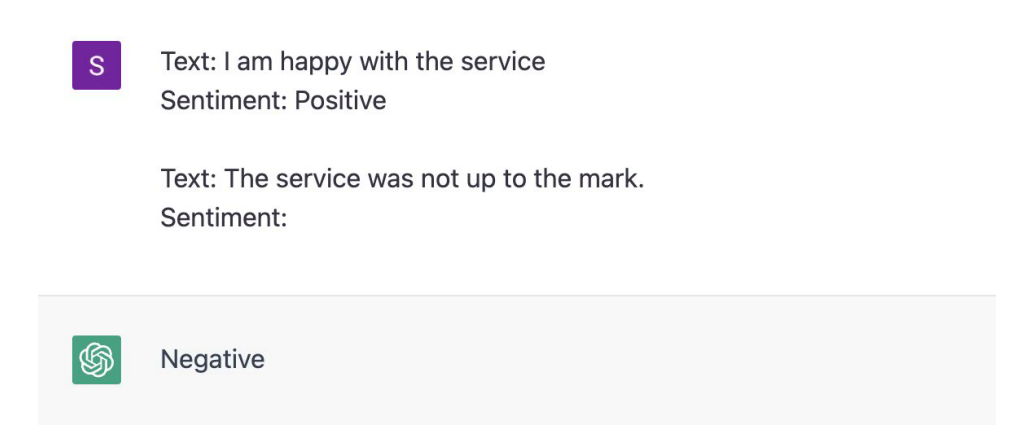
\includegraphics[width=\linewidth,keepaspectratio]{promptengg9}

{\tiny (Ref: Cohere https://txt.cohere.ai/generative-ai-part-1/)}

\end{center}		
		
\end{frame}

%%%%%%%%%%%%%%%%%%%%%%%%%%%%%%%%%%%%%%%%%%%%%%%%%%%%%%%%%%%
\begin{frame}[fragile]\frametitle{Length Control}

Specify a desired word count or character count as part of the prompt

\begin{center}
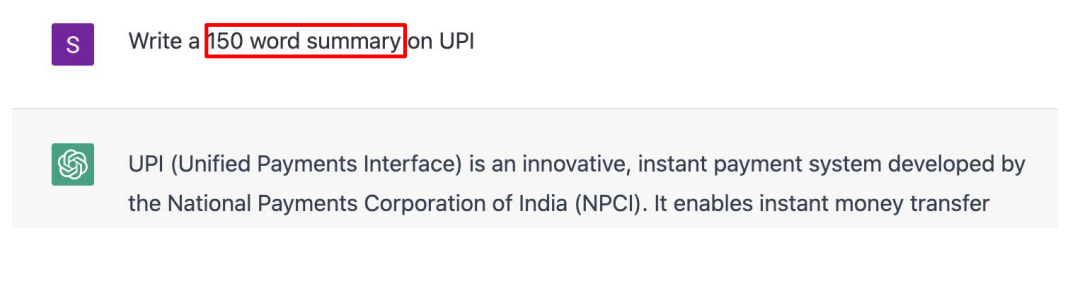
\includegraphics[width=\linewidth,keepaspectratio]{promptengg16}

{\tiny (Ref: Prompt Engineering Sudalai Rajkumar)}

\end{center}		

\end{frame}

%%%%%%%%%%%%%%%%%%%%%%%%%%%%%%%%%%%%%%%%%%%%%%%%%%%%%%%%%%%
\begin{frame}[fragile]\frametitle{Tone Control}

Specify specific words or phrases that indicate the desired tone

\begin{center}
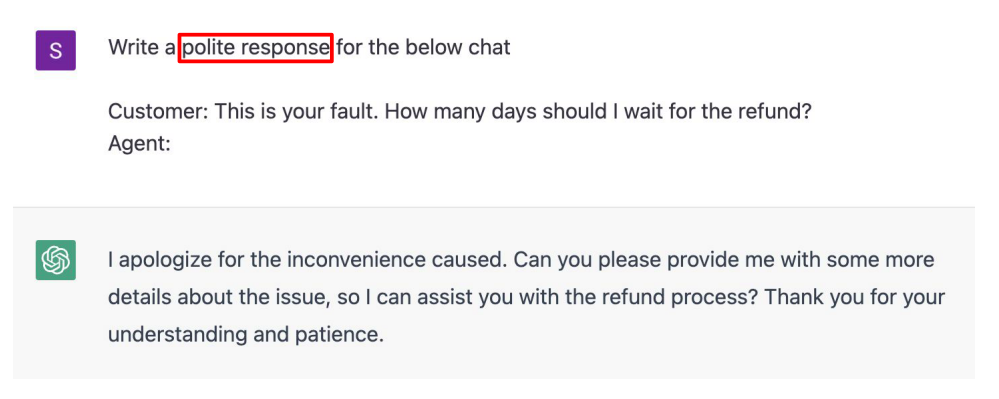
\includegraphics[width=\linewidth,keepaspectratio]{promptengg17}

{\tiny (Ref: Prompt Engineering Sudalai Rajkumar)}

\end{center}		

\end{frame}

%%%%%%%%%%%%%%%%%%%%%%%%%%%%%%%%%%%%%%%%%%%%%%%%%%%%%%%%%%%
\begin{frame}[fragile]\frametitle{Style Control}

Specify the desired writing style.

\begin{center}
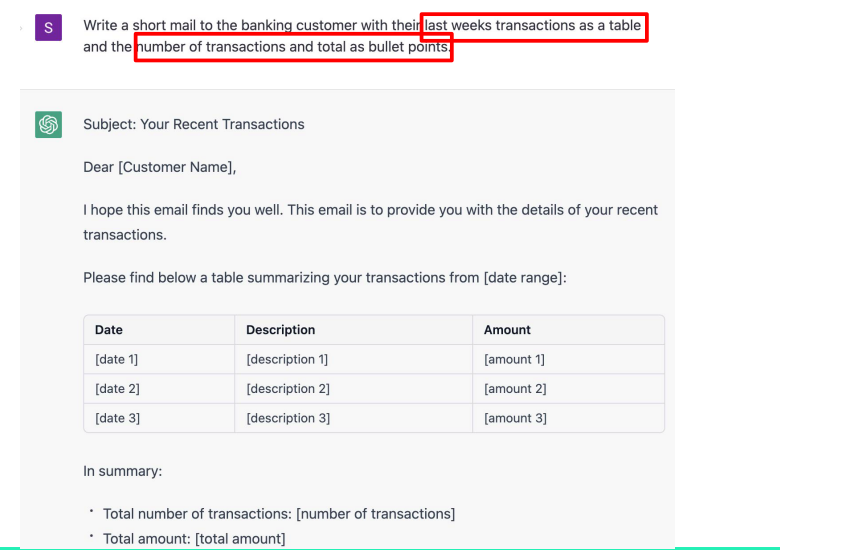
\includegraphics[width=\linewidth,keepaspectratio]{promptengg18}

{\tiny (Ref: Prompt Engineering Sudalai Rajkumar)}

\end{center}		
	
\end{frame}

%%%%%%%%%%%%%%%%%%%%%%%%%%%%%%%%%%%%%%%%%%%%%%%%%%%%%%%%%%%
\begin{frame}[fragile]\frametitle{Audience Control}

Specify the desired audience.

\begin{center}
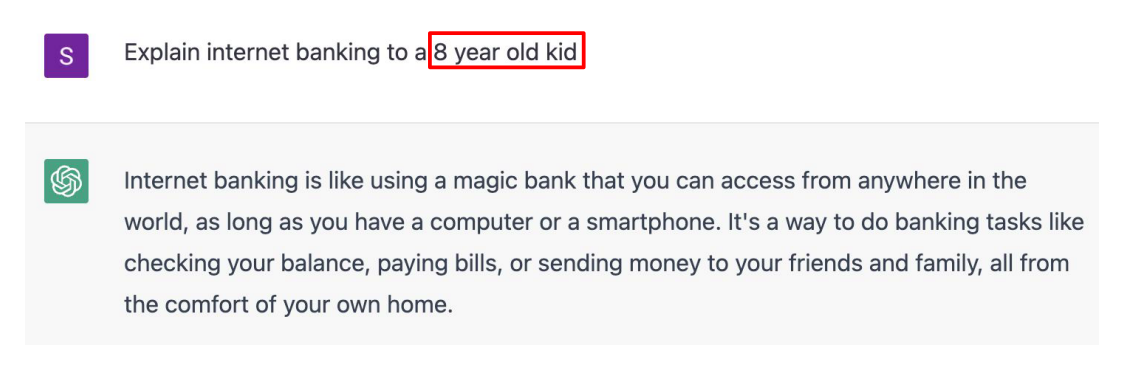
\includegraphics[width=\linewidth,keepaspectratio]{promptengg19}

{\tiny (Ref: Prompt Engineering Sudalai Rajkumar)}

\end{center}		

\end{frame}

%%%%%%%%%%%%%%%%%%%%%%%%%%%%%%%%%%%%%%%%%%%%%%%%%%%%%%%%%%%
\begin{frame}[fragile]\frametitle{Context Control}

Specify the information about the context.

\begin{center}
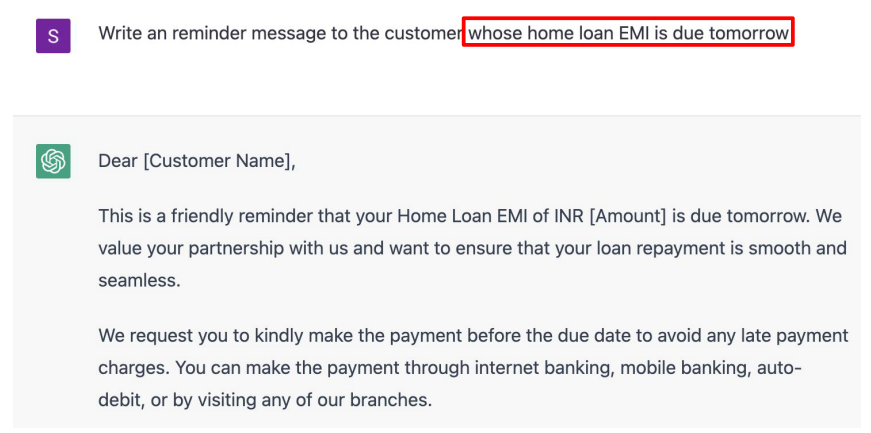
\includegraphics[width=\linewidth,keepaspectratio]{promptengg20}

{\tiny (Ref: Prompt Engineering Sudalai Rajkumar)}

\end{center}		

\end{frame}



%%%%%%%%%%%%%%%%%%%%%%%%%%%%%%%%%%%%%%%%%%%%%%%%%%%%%%%%%%%
\begin{frame}[fragile]\frametitle{Calling of Prompt}

\begin{lstlisting}
import openai
import os

from dotenv import load_dotenv, find_dotenv
_ = load_dotenv(find_dotenv())

openai.api_key  = os.getenv('OPENAI_API_KEY') # for langchain it does it automatically

def get_completion(prompt, model="gpt-3.5-turbo"):
    messages = [{"role": "user", "content": prompt}]
    response = openai.ChatCompletion.create(
        model=model,
        messages=messages,
        temperature=0, # this is the degree of randomness of the model's output
    )
    return response.choices[0].message["content"]
\end{lstlisting}
		
\end{frame}

%%%%%%%%%%%%%%%%%%%%%%%%%%%%%%%%%%%%%%%%%%%%%%%%%%%%%%%%%%%
\begin{frame}[fragile]\frametitle{Principles}

\begin{itemize}
\item Give clear and specific instructions
\item Give the model time to “think”
\end{itemize}
		
{\tiny (Ref: ChatGPT Prompt Engineering for Developers - Deep Learning AI)}
		
\end{frame}


%%%%%%%%%%%%%%%%%%%%%%%%%%%%%%%%%%%%%%%%%%%%%%%%%%%%%%%%%%%%%%%%%%%%%%%%%%%%%%%%%%
\begin{frame}[fragile]\frametitle{}
\begin{center}
{\Large Applications of Prompts}
\end{center}
\end{frame}

%%%%%%%%%%%%%%%%%%%%%%%%%%%%%%%%%%%%%%%%%%%%%%%%%%%%%%%%%%%
\begin{frame}[fragile]\frametitle{Text Generation}

\begin{center}
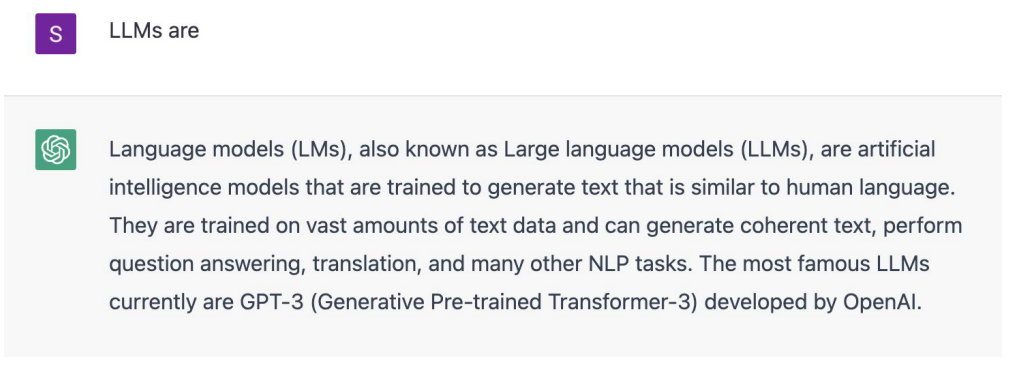
\includegraphics[width=\linewidth,keepaspectratio]{promptengg10}

{\tiny (Ref: Prompt Engineering Sudalai Rajkumar)}

\end{center}		
		


\end{frame}

%%%%%%%%%%%%%%%%%%%%%%%%%%%%%%%%%%%%%%%%%%%%%%%%%%%%%%%%%%%
\begin{frame}[fragile]\frametitle{Text Classification}

\begin{center}
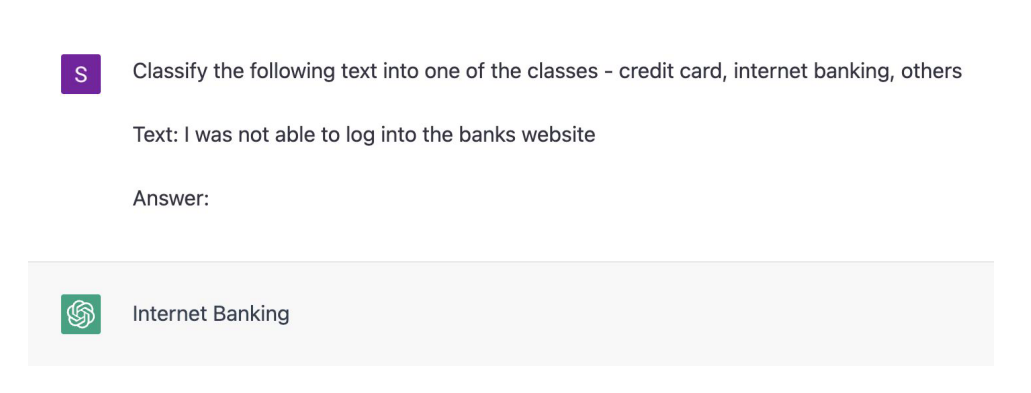
\includegraphics[width=\linewidth,keepaspectratio]{promptengg11}

{\tiny (Ref: Prompt Engineering Sudalai Rajkumar)}

\end{center}		
		


\end{frame}

%%%%%%%%%%%%%%%%%%%%%%%%%%%%%%%%%%%%%%%%%%%%%%%%%%%%%%%%%%%
\begin{frame}[fragile]\frametitle{Text Translation}

\begin{center}
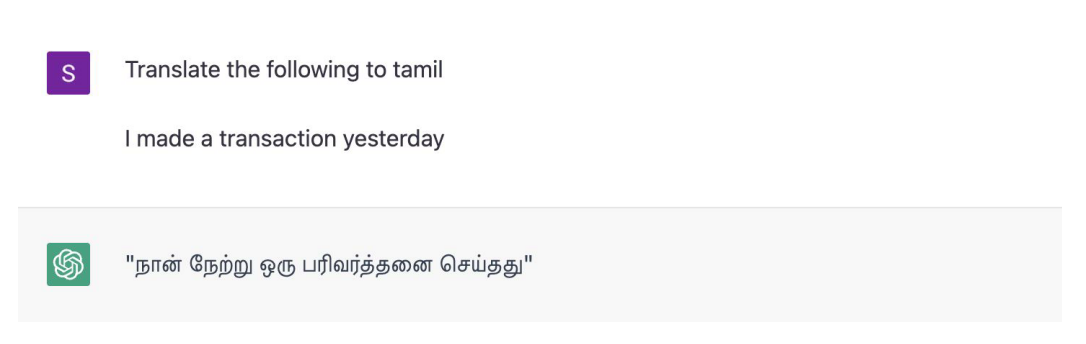
\includegraphics[width=\linewidth,keepaspectratio]{promptengg12}

{\tiny (Ref: Prompt Engineering Sudalai Rajkumar)}

\end{center}		
		


\end{frame}

%%%%%%%%%%%%%%%%%%%%%%%%%%%%%%%%%%%%%%%%%%%%%%%%%%%%%%%%%%%
\begin{frame}[fragile]\frametitle{Text Comprehension}

\begin{center}
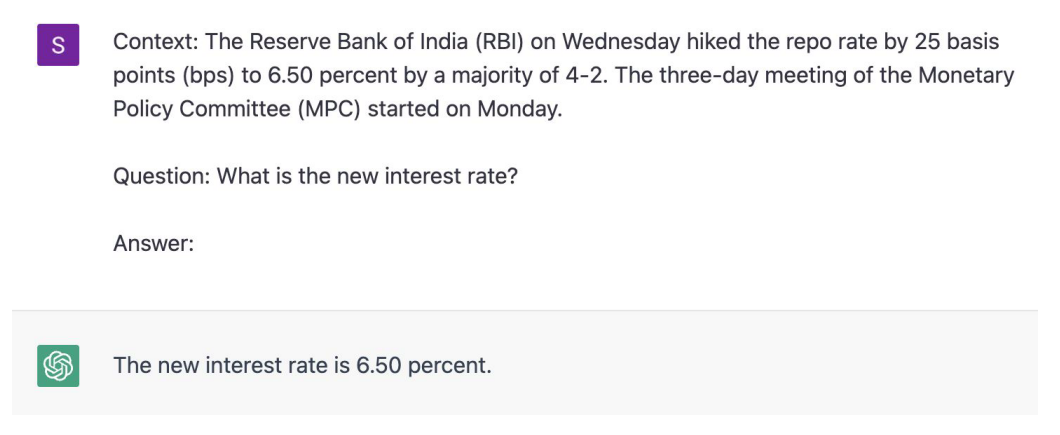
\includegraphics[width=\linewidth,keepaspectratio]{promptengg13}

{\tiny (Ref: Prompt Engineering Sudalai Rajkumar)}

\end{center}		
		


\end{frame}

%%%%%%%%%%%%%%%%%%%%%%%%%%%%%%%%%%%%%%%%%%%%%%%%%%%%%%%%%%%
\begin{frame}[fragile]\frametitle{Text Summarization}

\begin{center}
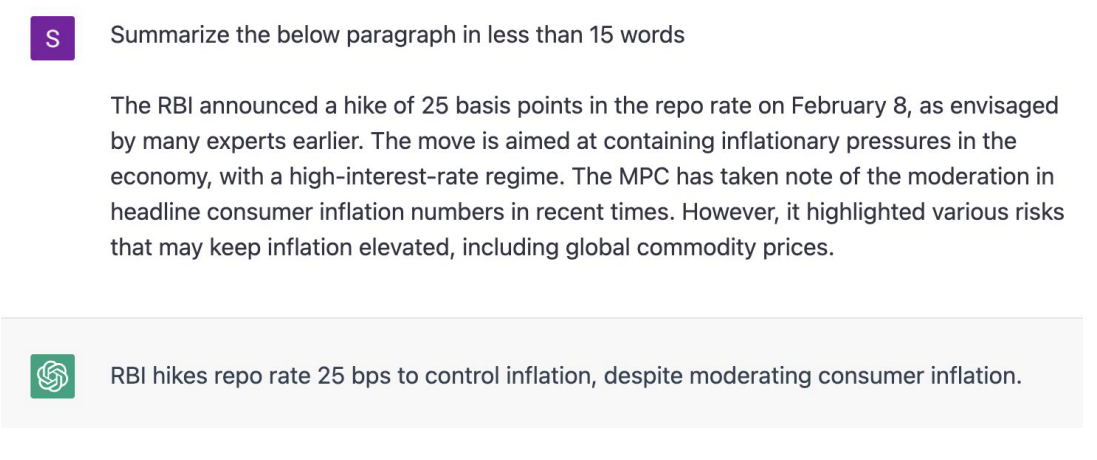
\includegraphics[width=\linewidth,keepaspectratio]{promptengg14}

{\tiny (Ref: Prompt Engineering Sudalai Rajkumar)}

\end{center}		
		


\end{frame}

%%%%%%%%%%%%%%%%%%%%%%%%%%%%%%%%%%%%%%%%%%%%%%%%%%%%%%%%%%%
\begin{frame}[fragile]\frametitle{Image Generation}

\begin{center}
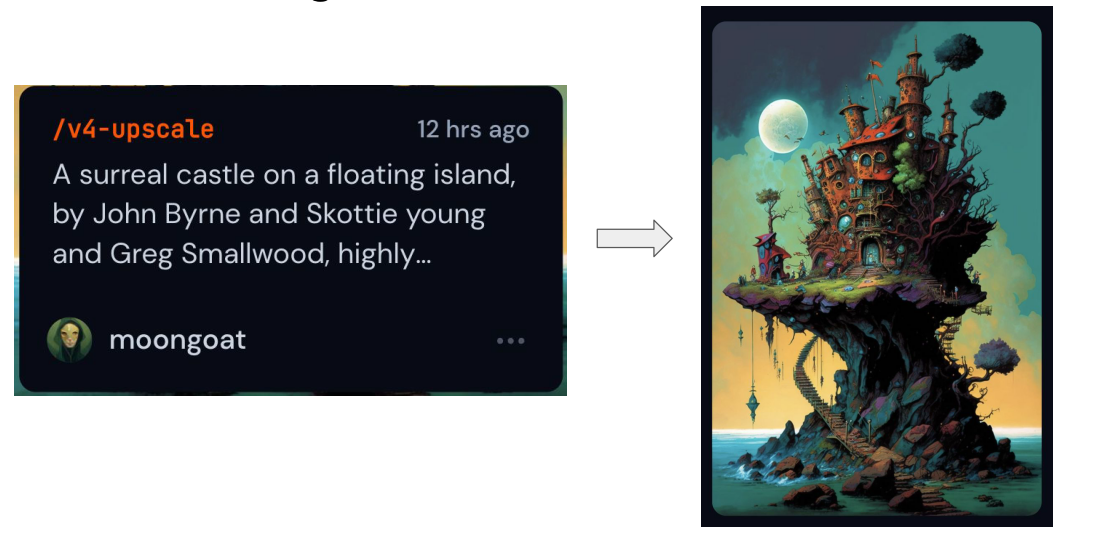
\includegraphics[width=\linewidth,keepaspectratio]{promptengg15}

{\tiny (Ref: Prompt Engineering Sudalai Rajkumar)}

\end{center}		
		
		
Models / Tools: Dall-E , Midjourney, Stable Diffusion



\end{frame}


%%%%%%%%%%%%%%%%%%%%%%%%%%%%%%%%%%%%%%%%%%%%%%%%%%%%%%%%%%%
\begin{frame}[fragile]\frametitle{For generating code using Codex}

Provide Codex with a prompt consisting of the following:



\begin{itemize}
\item  High level task description: Tell the model to use a helpful tone when outputting natural language
\item  High level context: Describe background information like API hints and database schema to help the model understand the task
\item  Examples: Show the model examples of what you want
\item  User input: Remind the model what the user has said before
\end{itemize}	 

{\tiny (Ref: https://microsoft.github.io/prompt-engineering/)}

\end{frame}

